\documentclass[11pt, oneside]{article} 
\usepackage{geometry}
\geometry{letterpaper} 
\usepackage{graphicx}
	
\usepackage{amssymb}
\usepackage{amsmath}
\usepackage{parskip}
\usepackage{color}
\usepackage{hyperref}

\graphicspath{{/Users/telliott_admin/Dropbox/Tex/png/}}
% \begin{center} 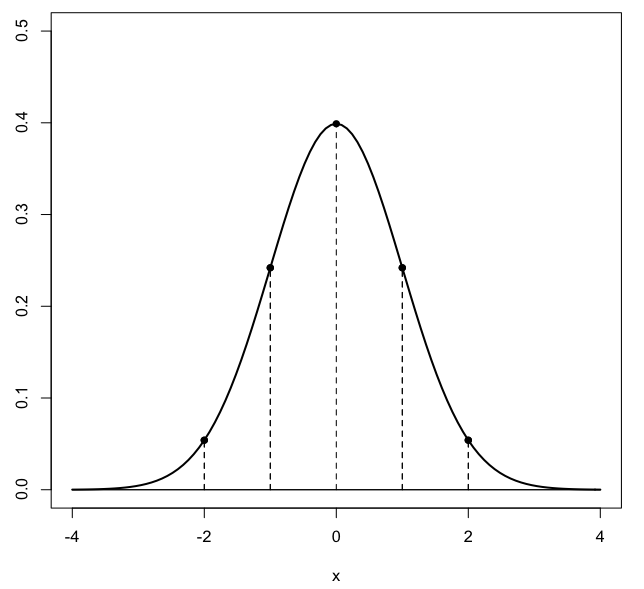
\includegraphics [scale=0.4] {gauss3.png} \end{center}

\title{Finite fields}
\date{}

\begin{document}
\maketitle
\Large

Suppose we start doing arithmetic with polynomials whose coefficients belong to a finite field.  Example:  $Z_7$ which can also be called $GF(7)$.

We construct such a field simply by doing all our arithmetic modulo $7$.  If a value is greater than or equal to 7, we divide by $7$ and set the value equal to the remainder.

For reference here is the multiplication table mod $7$ from earlier

\begin{verbatim}
  7
  1  |  0  1  2  3  4  5  6
  2  |  0  2  4  6  1  3  5
  3  |  0  3  6  2  5  1  4
  4  |  0  4  1  5  2  6  3
  5  |  0  5  3  1  6  4  2
  6  |  0  6  5  4  3  2  1
\end{verbatim}

and the power table

\begin{verbatim}
       1  2  3  4  5  6
  -----------------------
  1  | 1  2  3  4  5  6
  2  | 2  4  1  2  4  1
  3  | 3  2  6  4  5  1
  4  | 4  2  1  4  2  1
  5  | 5  4  6  2  3  1  
  6  | 6  1  6  1  6  1
\end{verbatim}

We will be doing all arithmetic mod $7$.  

For subtraction we can find the additive inverse of the second term and \emph{add} that to the first term.

\textbf{Additive inverses}
\[ 1 + 6 = 0 \  \text{mod} \  7 \]
\[ 2 + 5 = 0 \  \text{mod} \  7 \]
\[ 3 + 4 = 0 \  \text{mod} \  7 \]
So, for example, subtracting $3$ is the same as adding $4$

For division find a multiplicative inverse for the denominator and \emph{multiply} the numerator by that. Here is the multiplication table again:

\begin{verbatim}
  7
  1  |  0  1  2  3  4  5  6
  2  |  0  2  4  6  1  3  5
  3  |  0  3  6  2  5  1  4
  4  |  0  4  1  5  2  6  3
  5  |  0  5  3  1  6  4  2
  6  |  0  6  5  4  3  2  1
\end{verbatim}

In the table, you can see that $2 \times 4$ is equal to $1$, so $2$ and $4$ are multiplicative inverses.

\textbf{Multiplicative inverses}.
\[ 1 \ \text{ is its own inverse} \]
\[ 2 \times 4 = 8  = 1 \  \text{mod} \  7 \]
\[ 3 \times 5 = 15 = 1 \  \text{mod} \  7 \]
\[ 6 \times 6 = 35 = 1 \  \text{mod} \  7 \]
so $6$ is also its own multiplicative inverse.

The integers mod some number, say $n = 6$ or $n = 7$, with addition and multiplication defined in the standard way, form a finite ring, with additive and multiplicative identities.

However, to be a \textbf{field}, for each element, ${\{0,1,2,3,4,5,6\}}$, there must be a multiplicative inverse --- which may be the element itself.  If we lay out the multiplication table for arithmetic mod a prime number, then the row for each element contains all of the elements, including 1.  There are pairs of elements that when multiplied together give the multiplicative identity, 1.  Sometimes, the pair consists of an element which is its own inverse, say $6 \times 6 = 1$ (mod $7$).

We can also see multiplicative inverses in the power table:

\begin{verbatim}
       1  2  3  4  5  6
  -----------------------
  1  | 1  2  3  4  5  6
  2  | 2  4  1  2  4  1
  3  | 3  2  6  4  5  1
  4  | 4  2  1  4  2  1
  5  | 5  4  6  2  3  1  
  6  | 6  1  6  1  6  1
\end{verbatim}

However, there is something unusual about the power table.  If you look carefully you will see that only some of the numbers generate all the members of the field as a power of themselves.  $3$ and $5$ do, but $2$, $4$ and $6$ do not.

Kak:

\begin{quote}The number of elements of a finite field is called its order. A finite field of order q exists if and only if the order q is a prime power $p^k$ (where $p$ is a prime number and $k$ is a positive integer).\end{quote}

So not only prime numbers but prime powers $p^k$ can be used to construct fields.  If you look back at the table for arithmetic modulo $9$, you'll see that rows for integers which are co-prime to $9$ have all the elements, but the rows for $3$ and $6$ do not.

\begin{quote}In a field of order $p^k$, adding $p$ copies of any element always results in zero; that is, the characteristic of the field is $p$... The elements of the prime field of order $p$ may be represented by integers in the range $0, ..., p-1$.\end{quote}.

So for a finite field of order $q$ ($= 2^k$), the characteristic of the field is $2$.

\begin{quote}... the polynomial $X^q-X$ has all $q$ elements of the finite field as roots. The non-zero elements of a finite field form a multiplicative group.\end{quote}

So the business about polynomials apparently arises from the fact that we want to construct a Galois field for $2^8 = 256$, which is not prime, but is expressible as a prime power (of $2$).

\begin{quote}This group is cyclic, so all non-zero elements can be expressed as powers of a single element called a primitive element of the field. (In general there will be several primitive elements for a given field.)
\end{quote}

We will see much more about primitive elements.

To explain more about $X^q-X$:  this is an alternative way of writing $X^{q-1}$ and saying that if an element is the $q-1$ root of unity (i.e. $X^{q-1} = 1$) then it can generate all the elements of the field among its powers.

\end{document}